\chapter{Modeling}

\begin{figure}[hbtp]
	\centering
	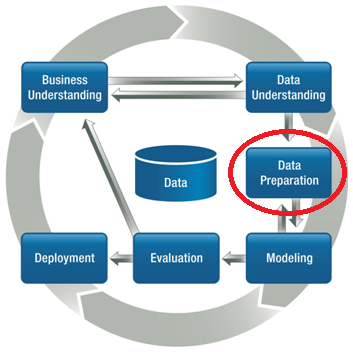
\includegraphics[width=0.5\textwidth]{./images/CRISPDM_3.png}
	\caption{CRISP-DM - Modeling}
	\label{CRISPDM_4}
\end{figure}

\section{Tecnica di Modeling}

\section{Rappresentazione del Modello}

\section{Valutazione del Modello}

\section{Ricerca}

\section{Test Design}

\section{Costruzione del Modello}

\section{Valutazione del Modello}

NAME
weka.classifiers.trees.FT

SYNOPSIS
Classifier for building 'Functional trees', which are classification trees  that could have logistic regression functions at the inner nodes and/or leaves. The algorithm can deal with binary and multi-class target variables, numeric and nominal attributes and missing values.

For more information see: 

Joao Gama (2004). Functional Trees.

Niels Landwehr, Mark Hall, Eibe Frank (2005). Logistic Model Trees.

OPTIONS
binSplit -- Convert all nominal attributes to binary ones before building the tree. This means that all splits in the final tree will be binary.

debug -- If set to true, classifier may output additional info to the console.

errorOnProbabilities -- Minimize error on probabilities instead of misclassification error when cross-validating the number of LogitBoost iterations. When set, the number of LogitBoost iterations is chosen that minimizes the root mean squared error instead of the misclassification error.

minNumInstances -- Set the minimum number of instances at which a node is considered for splitting. The default value is 15.

modelType -- The type of FT model. 0, for FT, 1, for FTLeaves, and 2, for FTInner

numBoostingIterations -- Set a fixed number of iterations for LogitBoost. If >= 0, this sets a fixed number of LogitBoost iterations that is used everywhere in the tree. If < 0, the number is cross-validated.

useAIC -- The AIC is used to determine when to stop LogitBoost iterations. The default is not to use AIC.

weightTrimBeta -- Set the beta value used for weight trimming in LogitBoost. Only instances carrying (1 - beta)\% of the weight from previous iteration are used in the next iteration. Set to 0 for no weight trimming. The default value is 0.
